% !TeX encoding = UTF-8
% !TeX spellcheck = fr_FR
% !TeX root = ../mythesis.tex
% !TeX program = pdflatex (build)
%%% TeXmaker : no 'magic comments' but set Root with Options > Set as master file

%useful stuff for what follows

\newcommand{\kbf}{\pmb{k}}
\newcommand{\vbf}{\pmb{v}}
\newcommand{\rbf}{\pmb{r}}

\graphicspath{{./}{./fig/}{./chap3_custom_st/fig/}}

\chapter{Optical generation and spectroscopy of arbitrary acoustic horizons}

\label{chap:generation_transonic_fluid}

The study of particle creation in the presence of highly curved spacetime has been a subject of interest for many years. The most famous example is the Hawking radiation \cite{hawking_black_1972}, which predicts the creation of particles from the vacuum in the vicinity of a black hole event horizon enabling the black hole 
to evaporate. The obvious difficulty to test this prediction experimentally is double. First, the blackness of such an object makes it hard to spot with a telescope meaning one have to rely rather on the peculiar behavior of visible object moving in the gravitationnal field of such a supermassive object. The optical observation of a black hole took almost one century since the first prediction of gravitationnal collapse by Subrahmanyan Chandrasekhar in 1920. It required 
the synchonization of nine telescope across the world to obtain an optical system whose optical aperture is the size the diameter of earth. the black body temperature of 

As mentionned in the previous chapter, the creation of a sonic horizon in a polariton fluid can lead to spontaneous emission of bogoliubov modes provided the downstream region collective excitation spectrum
exhibits negative energy modes. Furthermore, it was shown that the strength of the emitted signal depends strongly on the curvature of the horizon, or in other words, its steepness. To ensure that particle creation is in principle 
possible to be observed in the lab, one need to fully characterize the mean field of the fluid as well as locally probe its excitation spectrum. This chapter is dedicated to the description of the fully optical generation of arbitrary transonic fluids as well as the characterization of the excitation spectrum on both side of the horizon. 
The latter revealed the first measurement of negative energy modes in a supersonic quantum fluid, validating the possibility to observe particle creation in a polariton fluid.

The first part will focus on the generation of mean fields with arbitrary velocity profile through the shapping of the pump laser phase. In a second part, we will present the pump probe spectroscopy method used to locally measure the collective excitation spectrum as well
as the results obtained on several transonic fluids. The results obtained are reported in Ref ??

\section{Optical generation of arbitrary fluid velocity field}


Let us set the coordinates $x$ and $y$ to describe the microcavity plane. As explained in Chapter 2, translationnal invariance in the $xy$-plane ensure in plane momentum conservation along photonic polaritons excitation while the wavevectors along the
$z$ direction are fixed by the cavity and quantum well length. Furthermore, in this experiment the laser beam is set to be quasi resonant with the lower polariton branch. As a consequence, the transverse phase of the laser is directly imprinted on the polariton field.
Indeed, in the low wavevector limit, the lower polariton branch can be safely approximated by a parabola, namely :

\begin{equation}
    \omega_{LP}(\kbf) = \omega_{LP}^0 + \dfrac{\hbar k^2}{2m_{LP}}.
\end{equation}

The group velocity of a polariton is then $\vbf = \frac{\partial \omega_{LP}}{\partial k} = \frac{\hbar \kbf}{m_{LP}}= \frac{\hbar \kbf_p}{m_{LP}}=$ where $\kp$ is the in plane wavector of the pump laser.
In the case of a plane wave $\kp=\vec{\nabla}\theta(\rbf)$ where $\theta(r)$ is the spatial phase. This can safely be generalized to more complex spatial phase profile.
At the end, we obtain a direct link between the driving laser phase and the velocity of the fluid :

\begin{equation}
    \vbf = \dfrac{\hbar \vec{\nabla} \theta(\rbf)}{m_{LP}} .
\end{equation}

\subsection{Waterfall configuration}

A first realisation of a 1D acoustic black hole in a polaritonic system was done in \cite{nguyen_acoustic_2015} with the so called waterfall configuration. 
The setup was composed of a microcavity etched to be truly one dimensionnal and a defect was added in the middle of the wire to act as an external attractive potential and force the polariton flow to accelerate. The pump was only shone in the region before the defect. The downstream region of the flow was then made of polariton that propagate balistically and whose speed is fixed by the interaction energy
in the upstream region.
Eventhough this configuration provide a natural fluid acceleration, the horizon geometry depends greatly on the defect shape and can not be tuned easily.  Furthermore, the collective excitation spectrum and the presence of negative energy modes was not investigated which 
prevent to conclude on the nature of the signal observed in the experiment. In the present work, we present a different approach to generate such flows with an effective 1D fluid fully optically created as well as a full characterization of the Bogoilubov spectrum.

\subsection{Target velocity profile}
Before entering in consideration about whether the fluid cross a critical velocity or not the first task is to be able to generate a fluid that exhibits two homogeneous regions separated by a sharp transition and yielding two well defined velocities. 
To clarify, let us call the region before the transition the upstream region with velocity $v_{up}$ and the region after the transition the downstream region with velocity $v_d$.
To model this configuration, we arbitrary define a target velocity profile as follow : 

\begin{equation}
    v(x)= \frac{v_{d}-v_{up}}{2}\mathrm{tanh}(\frac{x-x_h}{w_h})+\frac{v_{up}+v_{d}}{2}
    \label{eq:target_velocity}
\end{equation}
where $x_h$ and $w_h$ are the position and width of the transition respectively. This profile is represented in \autoref{fig:target_velocity.pdf} a).
One can then verify that :

\begin{subequations}
    \begin{align}
    &\lim\limits_{x-x_h\ll-w_h} v(x) = v_{up},\\
    &\lim\limits_{x-x_h\gg+w_h} v(x) = v_{d}.
    \end{align}
\end{subequations}

\begin{figure}[h]
    \centering
    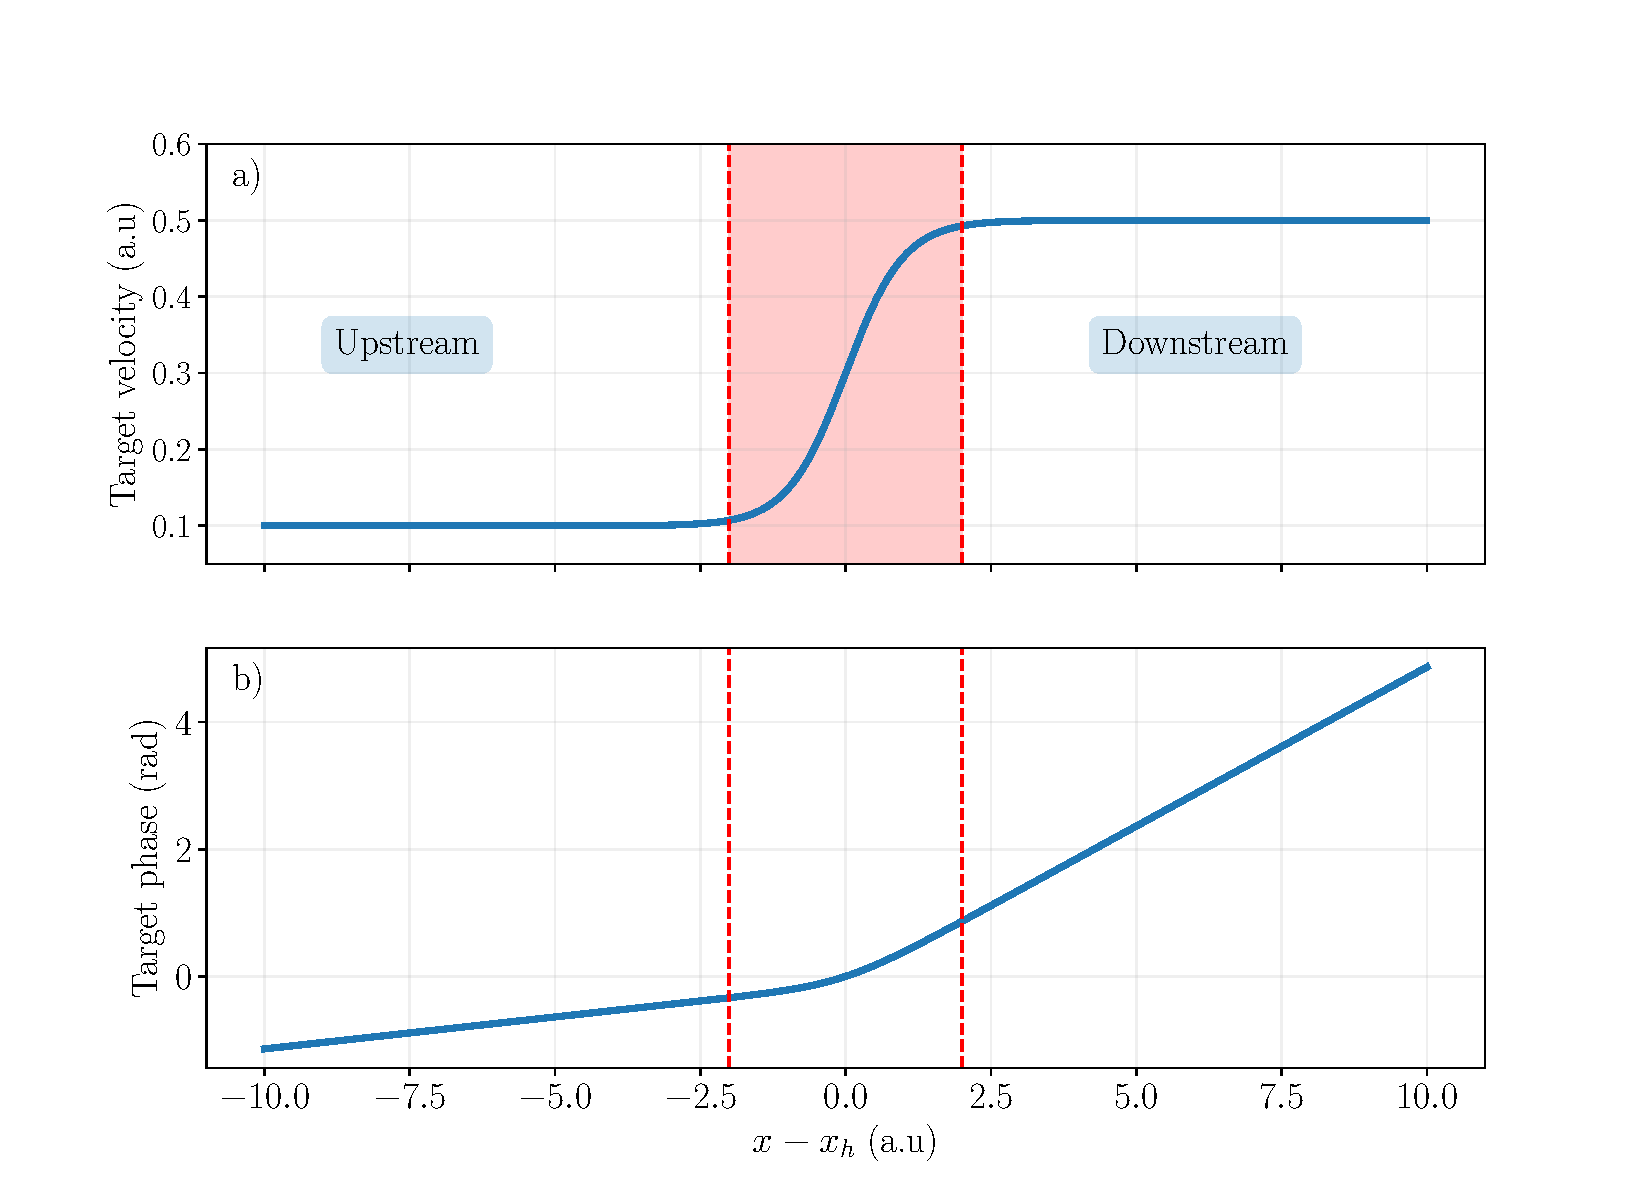
\includegraphics[width=1\textwidth]{chap3_custom_st/fig/target_velocity.pdf}
    \caption{ a) Target velocity profile for input parametes $v_{up}=0.1$, $v_{d}=0.5$, $x_h=0$ and $w_h=1$ in arbitrary units. The red shaded area represent the 
    transition region. b) Corresponding phase profile to be imprinted on the pump laser.}
    \label{fig:target_velocity.pdf}
\end{figure}

Such a velocity profile show a great flexibility in the choice of the upstream and downstream velocities as well as the steepness and the position of the transition. From 
this, one can determine the phase that must be imprinted on the pump laser to generate such a flow profile by simple integration of \autoref{eq:target_velocity}, which gives :

\begin{equation}
    \phi(x) = \dfrac{m_{LP}}{\hbar} \int v(x) dx = \dfrac{m_{LP}}{\hbar} \left( \dfrac{v_{d}-v_{up}}{2} w_h \mathrm{ln}(\cosh(\dfrac{x-x_h}{w_h}))+\dfrac{v_{up}+v_{d}}{2}x \right).
    \label{eq:target_phase_profile}
\end{equation}

The latter is plotted in \autoref{fig:target_velocity.pdf} b). The derivative of this curve at position $x$ gives the the local wavevector of the pump laser or in other words, this curve it represent directly a view side of the wavefront of the driving laser. Indeed, the wavefront is defined as the surface of constant phase of the beam. If we remind that the driving laser has also 
a wavevector along the $z$ direction fixed by the resonant conditions the isophase surfaces of the total laser phase  $\theta_{laser}$ are :

\begin{equation}
    \begin{align}
    \theta_{laser}(r)&=k_zz+\phi(x)=cst \\
                      &=\frac{2\pi n_{cav} }{\lambda_0}z+\theta(x)= cst,
    \end{align}
\end{equation}

which is inverted as $z\propto \phi(x)$. Making a fluid with the wanted velocity field then boils down to be able to imprint the phase \autoref{eq:target_phase_profile} on the laser that resonantly excite the fluid. As we will see in the next section, this can be done with a Spatial Light Modulator (SLM). 

\subsection{Wavefront shapping}

Controlling precisely the phase of a laser beam is a common but challenging task in optics. The most basic way to do it is by applying spatial filtering in the fourier plane of a lens.
The phase of the beam after a second collimating lens is then given by the covolution product of the beam phase and the mask inverse fourier transform. This method then show its limits when one wants to 
generate complex phase profile since its depend on the mask form. A way to overcome this problem is the use of Digital Micromirror Device (DMD) which is an array of micro-mirrors that can be individually controlled to reflect the light or not.
By putting this array in the fourier plan of a lens it is possible to create spatial filtering with arbitrary shapes. However, this method suffers from high losses and diffraction of the light on the individual mirrors that tend to 
add unwanted noise. This being said, DMD are very powerfull devices and allow to do a great amount of things at low cost. A wide range of possible methods are referenced in the great work \cite{wavefront_shapping}. 

\bigskip

\textbf{Spatial light modulator.} In this work, we use a Spatial Light Modulator (SLM) which is a liquid crystal display that can be used to modulate the phase of a laser beam. The principle is to apply a voltage on each pixel of the SLM to change the orientation of the liquid crystal molecules. 
The phase shift is then given by the difference of the optical path of light going through the different pixels as shown in \autoref{fig:SLM}. 

\begin{figure}
    \centering
    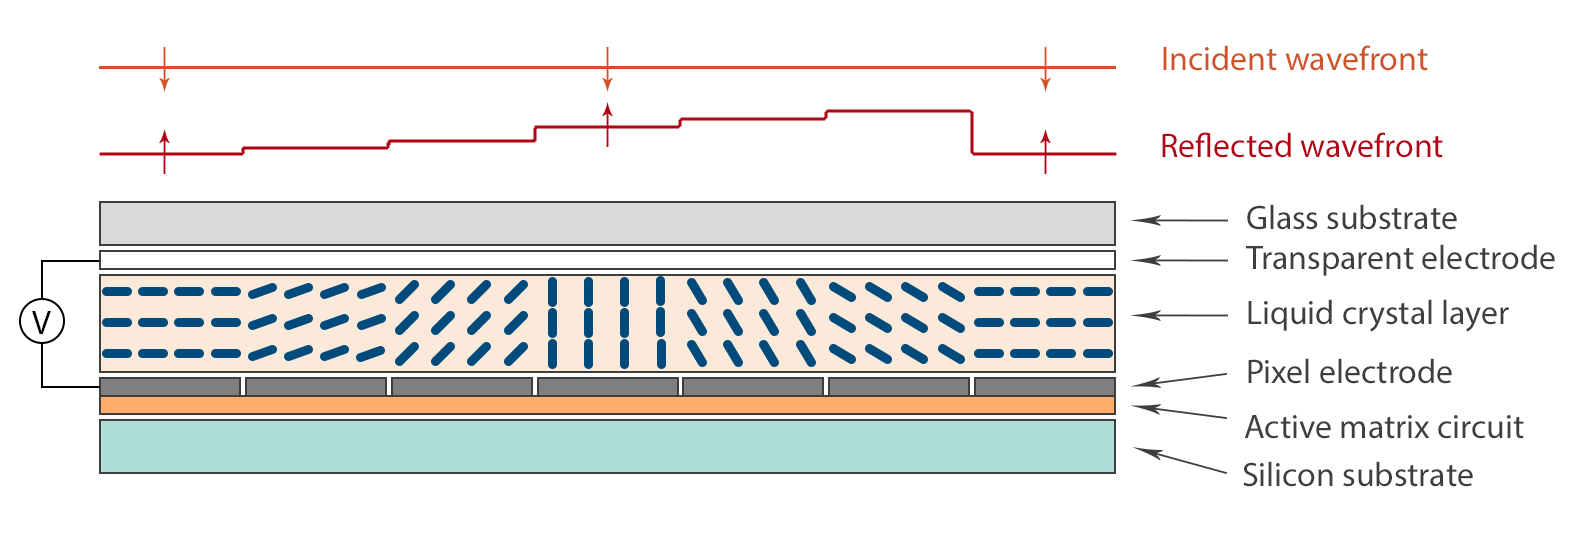
\includegraphics[width=1\textwidth]{chap3_custom_st/fig/SLMprinciple.png}
    \caption{Principle of a Spatial Light Modulator.}
    \label{fig:SLM}
\end{figure}

\noindent By shinning a flat phase collimated beam on the SLM which displays the target phase profile the beam gets reflected carrying the desired wavefront.
However the efficiency of the SLM is not perfect and whenever light is shone on it, some photons migth not see it and not be phase modulated. To overcome this difficulty,
we first write a blazed phase grating on the SLM screen on top of which the wanted profile is set. All the photons that did interact with the liquid crystals are then mostly diffracted on the first order of the grating. Doing so,
an efficiency of 60-70\% can be reached. This contrast with the usual 80\% usually claimed on manufacturer datasheets that actually correspond to the efficiency in all orders. A typical phase profile encoded on the SLM is shown
in \autoref{fig:SLM_profile}. A gray value of zero correspond to no shift while 255 corresponds to $2\pi$. The gray map corresponding to the target phase profile has been unwrapped for the sake 
of clarity and is shown in \autoref{fig:SLM_profile} c). The final gray map displayed on the SLM screen in represented in \autoref{fig:SLM_profile} e). 

\begin{figure}
    \centering
    \hspace{-1.4cm}
    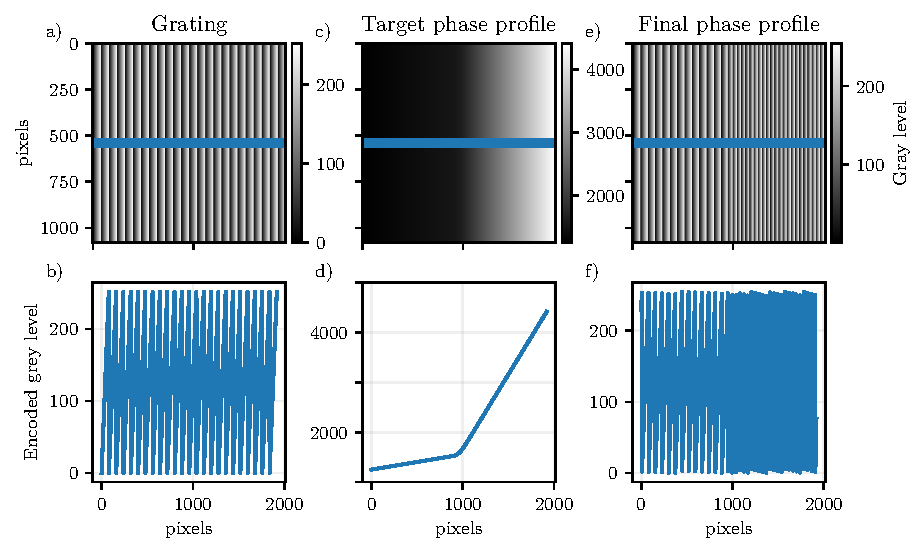
\includegraphics[width=1.1\textwidth]{chap3_custom_st/fig/slm_typical.pdf}
    \caption{Typical profile encoded on the SLM to generate the target velocity profile. a) Gray map of a phase blazed grating encoded on the SLM screen and b) corresponding cut in the 
    $x$ direction. c) Unwrapped grey map of the target phase profile and d) corresponding cut in the $x$ direction. e) Final gray map encoded on the SLM screen and f) corresponding cut in the $x$ direction. This map is the sum 
    of the blazed grating and the target phase profile modulus 255.} 
    \label{fig:SLM_profile}
\end{figure}

To imprint precisely the resulting wavefront in the cavity plane two $2f-2f$ optical telescopes are used in series to image the SLM screen with an overall demagnification of 1/130 while avoiding short focal lenght that would introduce optical aberrations.
An adjustable slit is placed in the fourier plane of the first telescope to filter out the unwanted diffracted orders. A simplified scheme showing how a typical fluid flow is created thanks to phase printing is shown in
To verify that the beam has the expected phase we use an usual off axis interferometry method. The principle is the following :
the beam whose phase is to be measured is recombined on a CCD camera with a flat phase reference beam. An angle is volontary introduced between the two beam to create an interference pattern on the camera plane. The phase difference between 
the two beams is then encoded in the size of the fringes and can be recovered by performing a fourier transform on the interferogram and demodulate the signal around the satellite peak created by the angle between the two beams \cite{liebling_complex-wave_2004}.
As an example, the measured phase corresponding to the mean field displayed in \autoref{fig:wavefront_shapping} b) is shown in \autoref{fig:phase_example}.
 
\begin{figure}
    \centering
    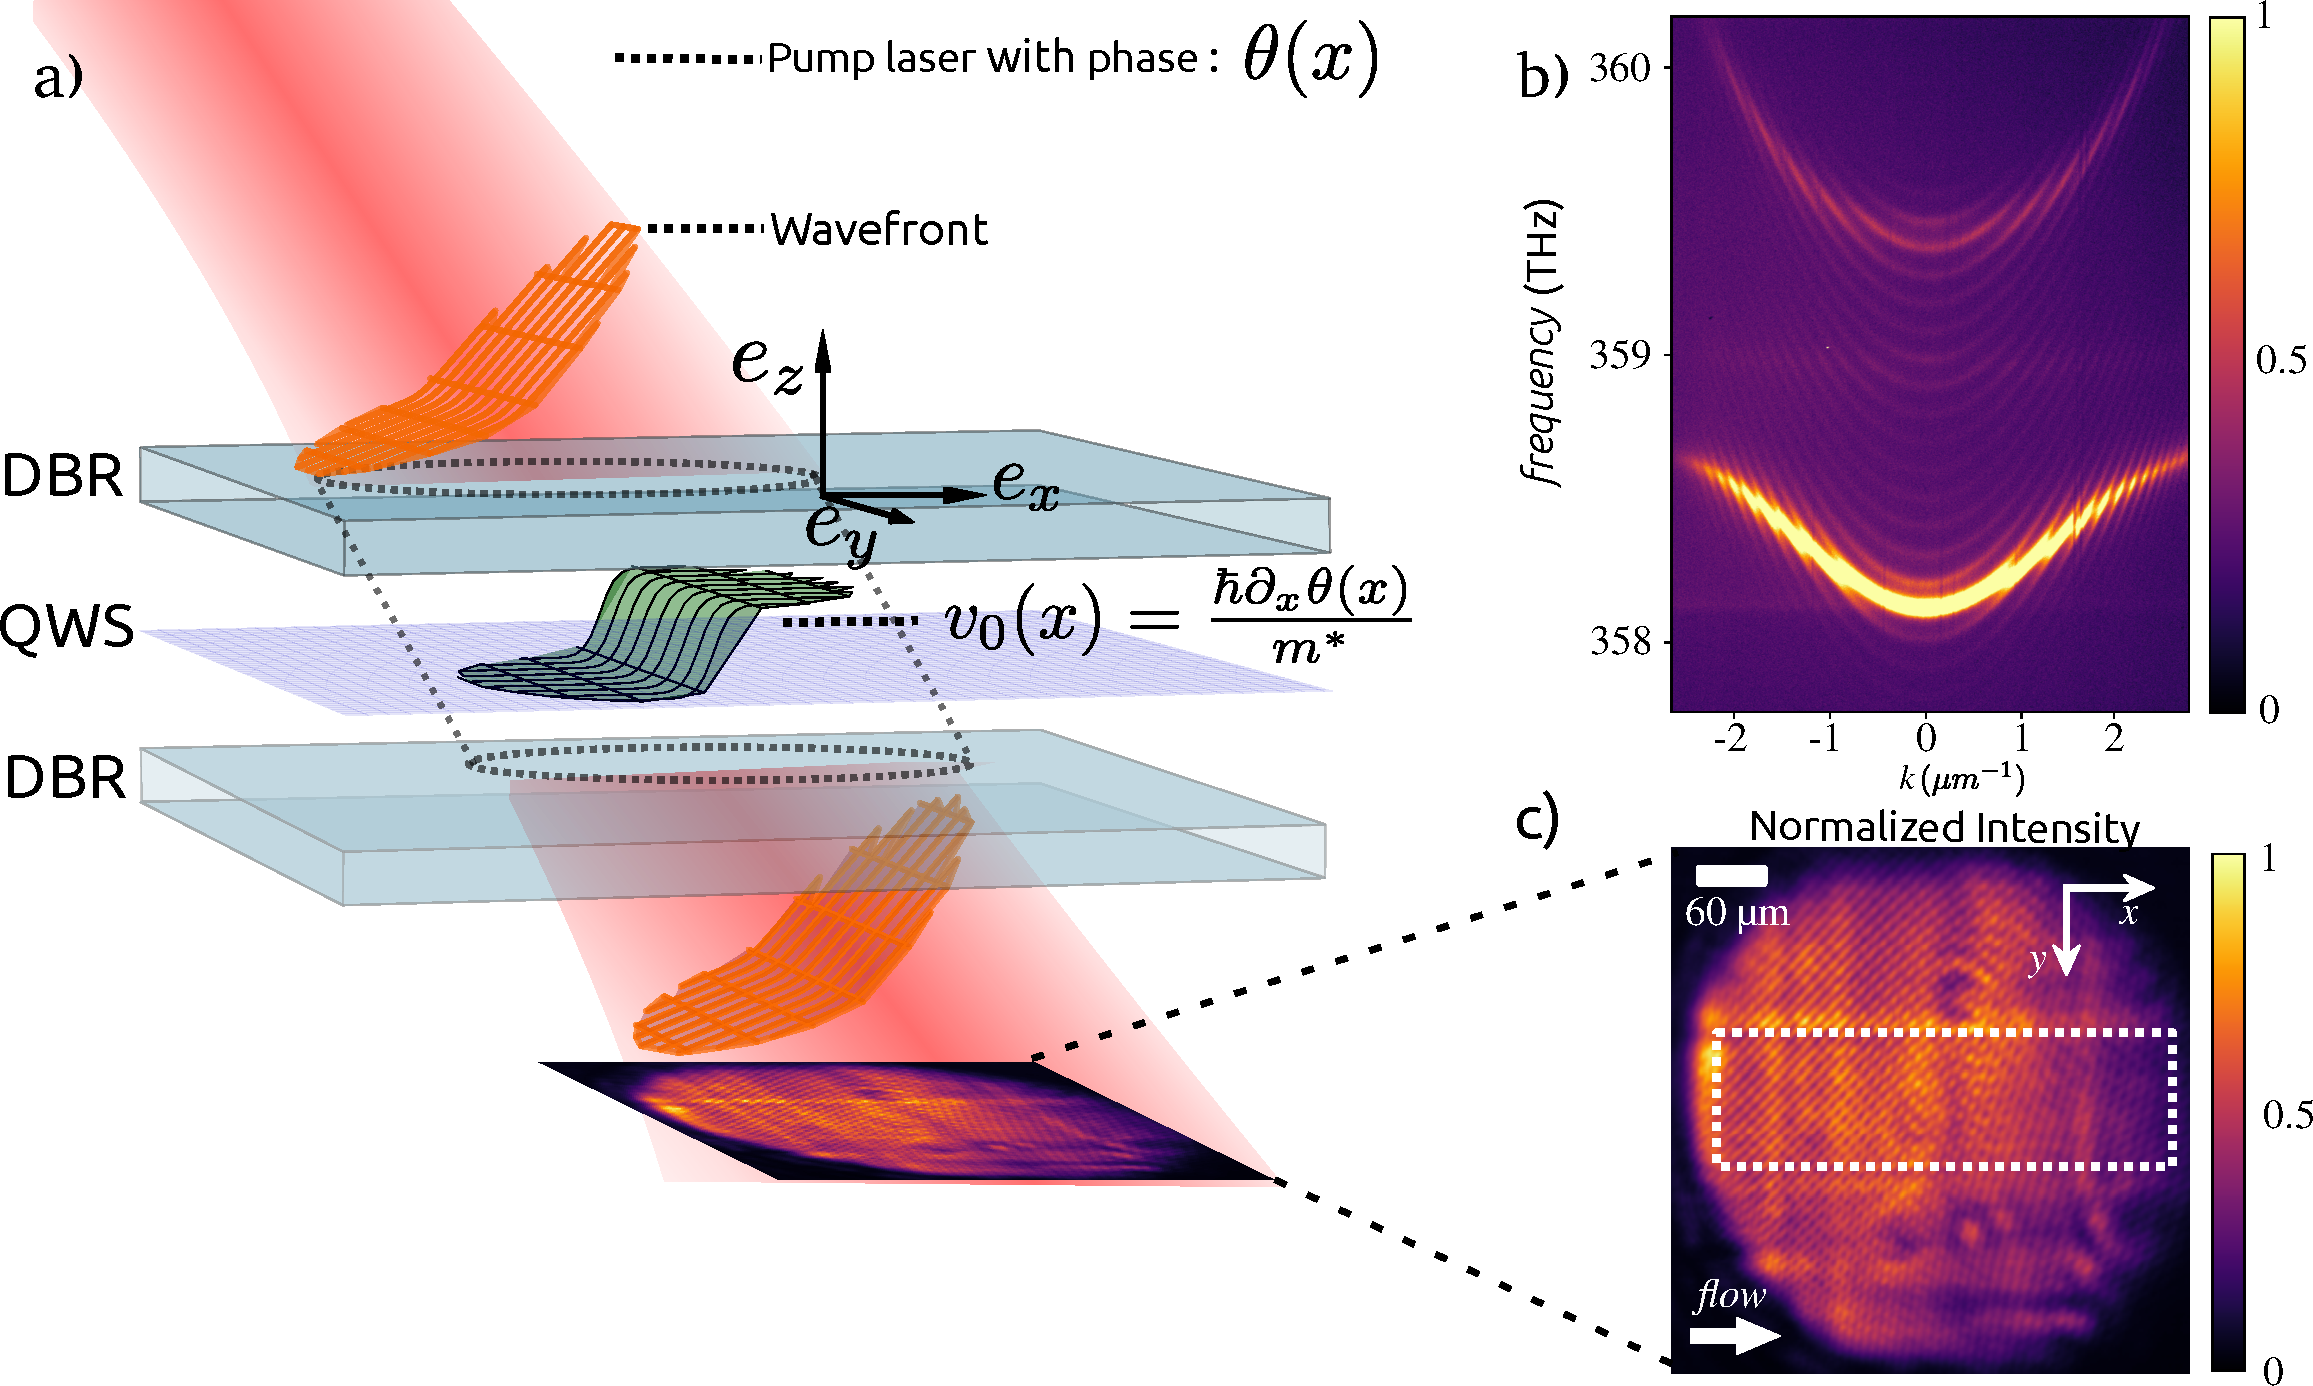
\includegraphics[width=1\textwidth]{chap3_custom_st/fig/wavefront_shapping.pdf}
    \caption{Simplified scheme of the generation of a transonic fluid. a) The pump laser is shapped with the target phase profile and sent on the microavity The corresponding fluid velocity field is represented by the black surface lying on the Quantum Wells (QWs). c) The outgoing photons are collected and the sample 
    plane is imaged on a CCD camera to obtain the fluid density map.  b) Measured Lower and Upper polariton dispersion at the working point $C6-D6$ at which the experiment was run. By fitting this dispersions,
    the effective LP mass can be extracted $\mlp= 7.0 \times 10^{-35}$ kg}
    \label{fig:wavefront_shapping}
\end{figure}


\bigskip 

\textbf{Controlling the local intensity}. Being able to modifiy on demand the intensity of the pump laser along with the phase is also crucial since the polariton fluid density and thus the regime of collective excitation 
depends on the input intensity as explained in ??. Notably, if the operating point of the fluid is set at the turning point of the bistabilty loop it exhibits a linear collective excitation spectrum and the speed of sound is directly 
linked to the detuning of the laser with respect to the lower polariton branch as $gn+g_rn_r=\delta(k_p)$. More generally, the possibility to move on the higher branch of the bistability enable to control the gap opening in the bogoliubov spectrum from a linear spectrum to masslike one. 
Once again, this can be done with the SLM by changing locally the height of the phase grating under the target phase profile. This will reduce the amount of photons sent in the first diffracted order. This method is widely used to
create top hat intensity profiles and is of high interest in metrology or cold atoms experiments to reduce systematic effects \cite{top_metrology_2018}.

\bigskip


\begin{figure}
    \centering
    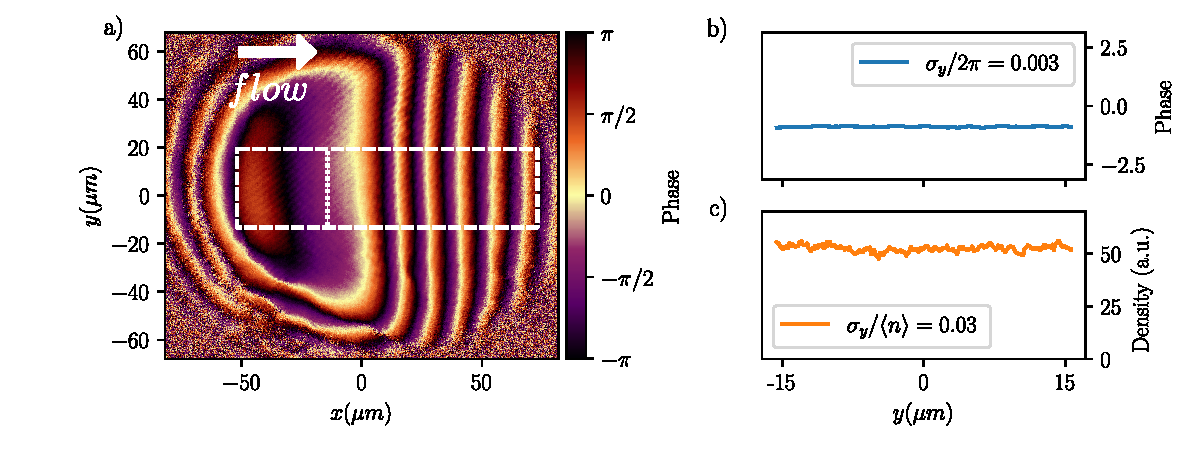
\includegraphics[width=1\textwidth]{chap3_custom_st/fig/phase_example.pdf}
    \caption{a) Measured phase of the mean field shown in \autoref{fig:wavefront_shapping}.The curvature present in the upstream region is due to the non linear self focusing. The region
    on interest in which we assume translationnal invariance is represented by the white dashed rectangle. b)  Ct of the phase in the $y$ direction represented by the dotted white line in the rectangle. The variation to the phase with respect
    to $2\pi$ are equal to 0.3\%. c) Cut of the intensity of the mean field in the $y$ direction at the same location than b). The corresponding relative intensity variation is equal to 0.3\%.}
    \label{fig:phase_example}
\end{figure}

To summarize, it is possible to generate fluid with arbitrary density and velocity flow by shapping the pump laser both in phase and intensity with a single device, namely, a Spatial Light Modulator. This method is very flexible and full optical
which is a great advantage since it allow to change the fluid property on the fly. 

\subsection{Effective 1D polariton fluid}

So far, the description of the fluid both in velocity and density was one dimensionnal despite the fluid is actually a 2D system. This assumption
rely on the fact that the fluid wavefunction is invariant under translation in the $y$ direction in a given region of interest represented by the white dashed rectangle of \autoref{fig:phase_example}. This area is approximatively $130 \mu m$ long and $30-40 \mu m $ large. 
A cut of both the phase and density in the direction orthogonal to the propagation are shown in \autoref{fig:phase_example} b) and c). Periodic modulations are present because of back reflection on the protection screen of the camera sensor and are present even without passing through the sample. These modulation can be removed
upon fourier filtering which allow to compute the variation of the phase with respect to $2\pi$,  $\sigma_y^{ph}/2\pi$= 0.3\% as well as the relative intensity variation $\sigma_y^I/\langle I \rangle$ =3\%. As a consequence,
we can safely assume that the fluid is effectively 1D in the region of interest. This contrats with the work \cite{nguyen_acoustic_2015} previously mentionned. In the present configuration, the shape of the horizon is fixed by the phase of the exciting laser and can be tuned as will which is crucial to
study the effect of the horizon steepness on the emitted signals. Moreover, the presence of the pump laser in the downstream region brings a double advantage. First, the velocity of the fluid can be changed and doesn't depend on the interaction energy of the upstream region allowing to study many fluid configurations.
Secondly, this experiment doesn't suffer from the exponential density decay that come with ballistic propagation \cite{long_range_ballistic_2013}. As a consequence, it is possible to probe the collective excitation spectrum in any region of the fluid with a high resolution pump probe spectroscopy method that we will describe in the next section. The signal 
provided by this method depends on the response of the system to a weak perturbation. It is hence somehow proportionnal to the interaction energy of the fluid $gn$ and better suited to pumped fluid \cite{claude_high-resolution_2022}.

\section{Experimental spectroscopy of the collective excitation spectrum}

The analog of the Hawking radiation in a polariton fluid is the spontaneous emission of Bogoliubov modes from the horizon. When the system is operating at the turning point of the bistability the Bogoliubov spectrum 
is gapless and linear which enable to define a speed of sound $c_s = \sqrt{\hbar g n /\mlp}$ and speak without ambiguity of sonic excitation in the low wavevector limit. In this regime, the condition to observe negative energy modes coincide with the fluid being supersonic as explained in the previous chapter. 
However, creating a stable fluid at the turning point is quite challenging and the measurement of the spectrum linearity require experimental techniques that are hard to implement on a moving fluid \cite{claude_phd}. Nevertheless, linearity is not mandatory to observe Hawking radiation since 
it only requires the mixing between positive and negative energy modes which can be achieved without operating at the turning point. Besides, a gap opening in the Bogoliubov brings new physics on the table since it widen the study of quasi-particles creation to the case of massive particles. In this
section we discard the necessity to have sonic excitations and measure the presence of negative energy modes in a wide range of fluid configuration exploring different asymptotic velocities and horizon steepness.

\begin{figure}[h]
    \centering
    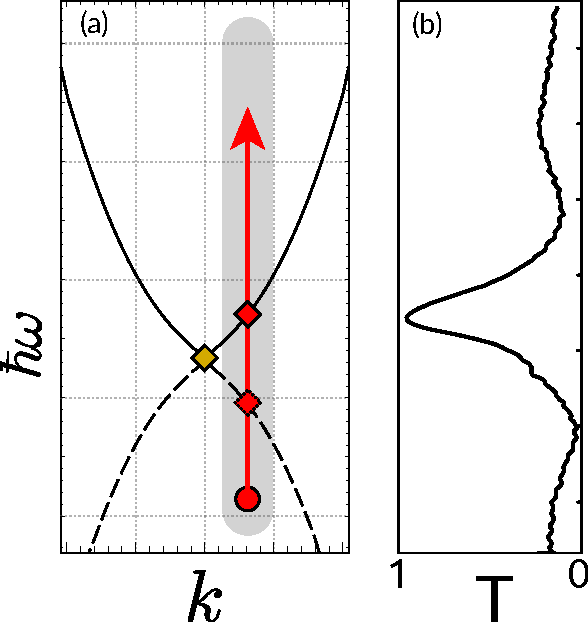
\includegraphics[width=0.3\textwidth]{chap3_custom_st/fig/setup_bogoliubov.pdf}
    \caption{Simplified scheme of the pump probe spectroscopy method. a) At a given in plane wavevector represented by the red arrow, the probe frequency is scanned around the mean field frequency and is transmitted when it resonate with the bogoliubov branch. b) Typical transmission spectrum of the probe at the wevevector of a).}
    \label{fig:setup_bogo}
\end{figure}


\subsection{High resolution pump-probe spectroscopy method}

\label{sub:high_resolution_spectroscopy}

The measurement of the collective excitation spectrum consists in scanning the mean field resonance by looking at the transmission of a weak probe laser at the different incidence angles. First, polariton fluid is created with a driving laser as described in the previous section. A probe laser is then sent on the sample with a well defined incidence corresponding to an in plane wavevector as explained in \autoref{sec:photon}. The frequency of 
the probe is then scanned around the mean field frequency. When the perturbation frequency matchs these of the collective excitation, the probe create perturbations in the fluid with same energy and wavevector that ultimately escape the sample as photons. Frequency scans are then repeated for different incidence angles providing each time a transmission spectrum of the probe as shown in \autoref{fig:setup_bogo}. 
To make sure that we stay in the weak perturbation regime the intensity of the probe is set two order of magnitude below the pump. To collect only the signal emitted in the perturbation mode, a tunable pinhole is placed in the Fourier plane of the collection path and track the probe in-plane wavevector position to filter out the unwanted photons. Finally, the probe intensity is modulated at $f_{mod}$ in order to isolate its transmission from the very strong signal of the pump. The remaining ligth is then sent on
a photodiode connected to a Spectrum analyzer that demodulates the signal at $f_{mod}$ to obtain the transmission spectrum. At the end, all the scans are put together to reconstruct the full collective excitation spectrum as typically shown in \autoref{fig:homogeneous_fluid_bogo}.



\section{Experimental setup}
The setup used in this experiment is shown in \autoref{fig:set_up}. The sample is a microcavity consisting of three InGaAs quantum wells sandwiched between two highly reflecting planar GaAs-AlGaAs Bragg mirrors.
The quantum wells, separated by GaAs barriers, are located at the three antinodes of the cavity, which has a finesse on the order of 3000. A complete map of this sample 
 can be found at the end of this manuscript in \autoref{fig:sample_map} along with exciton-photon detuning measurements. This map enable to perform an experiment over several days at the same working point and overcome the problem due to daily cooling and warming procedures imposed by the open cycle cryostat. Furthermore, despite rigourous and exhaustive
 characterization of the sample, the quality of certain measurement can be substancially enhanced by looking phenomenologically the right working point fitted to the experiment. This being said, the experiment described in this chapter was run on the working point $C5-D6$.
 The set up is divided in three main paths, the pump path, the probe path and the collection path.


 \begin{itemize}
    \item The pump path represented by the blue box is used to create the stationnary states of the experiment. The polariton fluid is generated by a circularly polarized CW Ti:sapphire laser with a sub-MHz linewidth. This laser can be precisely frequency tuned around the LP resonance energy centered around 836 nm in our sample. An AOM 
    together with a Proportionnal-integral-derivative feedback on the AOM driving RF are used to stabilize the laser intensity and make sure the experiment is constantly runned at a single fluid density.
    The stabilized Gaussian beam is reflected on the spatial light modulator (SLM) which imprints the target phase $\theta_\mathrm{p}(x)=\int v_0(x)dx$ that determines the fluid velocity $v_0(x)$ at each point. The SLM plane is imaged in the plane of the cavity with two focal-length matched telescopes ($2f-2f$ configuration).
    \item The probe path represented by the red box is used to measure the collective excitation spectrum. The probe is another tunable CW Ti:sapphire laser with. The probe is sent on the sample with a well defined incidence angle controlled by another SLM on which a tunable step blazed grating is imprinted. The frequency of
    the laser is scanned over $\SI{220}{\giga\hertz}$ around the mean field frequency and monitored by a high resolution wavemeter. An AOM and a Proportionnal-integral-derivative feedback are also used to both stabilize the intensity along the scan and apply a $f_{mod}=\SI{5}{\mega\hertz}$ intensity modulation.
    \item The collection path located after the sample is used to collect the signals emitted by the fluid. A microscope objective send the outgoing field on a 50:50 BS. One part is directed to an optical system to make the image both in real and momentum space of the field. For both lasers, a pick-up is made after their respective AOM to have a phase reference and perfom off axis interferometry measurement. Another part is sent to the apparatus described in \autoref{sub:high_resolution_spectroscopy} to measure the transmission spectrum of the probe. The tunable
    pinhole is made with a DMD placed in the fourier plan of a lense that send only photons arriving at the position of the pinhole to the collection photodiode.
 \end{itemize}

\textbf{k-space filtering.} In order


 \begin{figure}
    \centering
    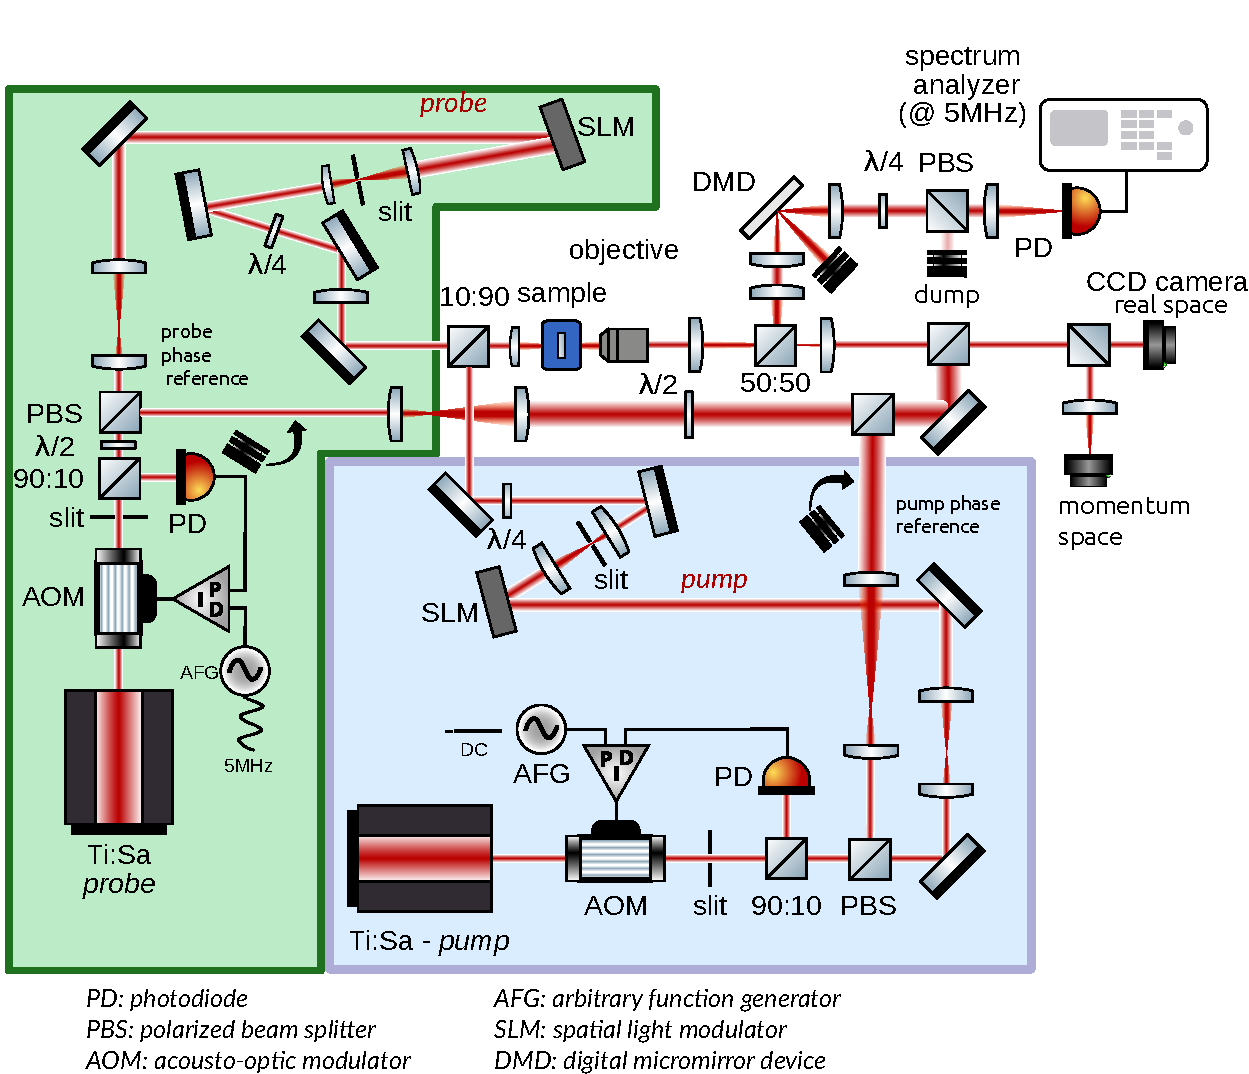
\includegraphics[width=1\textwidth]{chap3_custom_st/fig/set_up_spacetime.pdf}
    \caption{Experimental setup}
    \label{fig:setup}
\end{figure}





\section{Experimental results}

\subsection{Homogeneous fluid}

To begin with, we first create homogeneous fluid with a non zero velocity to see the effect of the doppler shift on the collective excitation spectrum. 